\documentclass[onecolumn, 11pt]{IEEEtran}
\IEEEoverridecommandlockouts
% The preceding line is only needed to identify funding in the first footnote. If that is unneeded, please comment it out.
\usepackage{cite}
\usepackage{amsmath,amssymb,amsfonts}
% \usepackage{algorithmic} % not used; enable if you add an algorithm environment
\usepackage{booktabs}
\usepackage[a4paper, margin=1.2in]{geometry}
\usepackage{graphicx}
\usepackage{textcomp}
\usepackage[hidelinks]{hyperref}
\usepackage{xcolor}
% \usepackage[flushleft]{threeparttable} % not used
\usepackage{caption}
\captionsetup{
    labelfont=bf, % Makes 'Table I' or 'Figure 1' bold
    labelsep=colon % Uses a colon instead of default formatting
}
\usepackage{tikz}
% \usepackage{svg} % not used; our figures are PDFs (svg needs --shell-escape + Inkscape)
\usepackage{float}
% \usepackage{multirow} % not used
\usetikzlibrary{fit,positioning,arrows.meta,shapes.misc,calc,backgrounds}
% NOTE: do not also load natbib here; it conflicts with the cite package and with IEEEtran.bst.
\DeclareMathOperator*{\argmax}{arg\,max}
\def\BibTeX{{\rm B\kern-.05em{\sc i\kern-.025em b}\kern-.08em
    T\kern-.1667em\lower.7ex\hbox{E}\kern-.125emX}}
\begin{document}

\pagestyle{plain}

\title{Assertion and Question Developer for Agentic Questionnaire Development}

\author{
\begin{minipage}{0.45\textwidth}
\centering
\IEEEauthorblockN{Lanre Oriowo}\\
\IEEEauthorblockA{\textit{Ludwig-Maximilian-University}\\
Munich, Germany \\
L.Oriowo@campus.lmu.de}
\end{minipage}
\and
\hfill
\begin{minipage}{0.45\textwidth}
\centering
\IEEEauthorblockN{Rudraksha Samdhani}
\IEEEauthorblockA{\textit{Ludwig-Maximilian-University}\\
Munich, Germany \\
Rudraksha.Samdhani@campus.lmu.de}
\end{minipage}
}

\maketitle

\begin{abstract}
    Designing high-quality survey items is expert-intensive, slow, and difficult to reproduce, which limits the pace of empirical work in computational social science. We investigate how far prompt engineering alone, without any fine-tuning, can drive an open-weight large language model to generate survey items that adhere to a formal survey-design framework. We implement a three-step design method, in which a raw indicator is mapped to a basic concept and a semantic structure, then to a declarative assertion, and finally to a respondent-facing question, as a two-agent pipeline built on a 9-billion-parameter model served with constrained JSON decoding. We evaluate the pipeline against a hand-built gold set of 115 items spanning 22 basic concepts, using a dual protocol that separates framework adherence, measured as exact match against the taxonomy, from semantic fidelity, measured with a large language model acting as a judge. Across six controlled prompt-engineering iterations, concept-identification accuracy rises from 57 to 77 percent and semantic-structure accuracy from 51 to 76 percent, with both labels jointly correct on 74 percent of items. An external 72-billion-parameter judge confirms that generated questions are semantically faithful, scoring 4.56 out of 5 on average with all items rated at least 4, even though only about 17 percent match the reference wording exactly. Comparing the model judging its own outputs against the external judge reveals a systematic self-grading bias of roughly 0.43 points. Our results show that framework-grounded prompt engineering reaches a strong baseline without training, and our error analysis identifies rare concepts, such as norms and policies, as the main remaining failure mode.
\end{abstract}

\begin{IEEEkeywords}
survey methodology, large language models, prompt engineering, question generation, structured decoding, LLM-as-a-judge, computational social science
\end{IEEEkeywords}

\tableofcontents

\section{Introduction}
Surveys are a primary instrument of empirical social science, yet the quality of the data they produce is bounded by the quality of their individual items. Designing items that are valid, unambiguous, and comparable across studies is a specialized craft: it requires domain expertise, familiarity with measurement theory, and repeated expert review \cite{groves2009survey}. This process is slow, costly, and difficult to reproduce, which constrains the pace of large-scale and cross-national research in computational social science, where hundreds of indicators may need to be turned into well-formed questions.

A substantial body of survey methodology argues that item construction should not be ad hoc but should follow an explicit procedure that separates the concept being measured from its linguistic realization. In particular, the three-step design method decomposes item construction into (i) identifying the \emph{basic concept} an indicator refers to together with its \emph{semantic structure}, (ii) formulating a declarative \emph{assertion} that expresses that concept in the prescribed structure, and (iii) transforming the assertion into a respondent-facing \emph{request for an answer}, that is, a survey question with response options \cite{saris2014design}. This framework grounds item design in a formal taxonomy of concepts and structures, which makes the output theory-consistent and, importantly for our purposes, checkable against a reference standard.

Large language models (LLMs) are natural candidates to automate this procedure: they are fluent, follow instructions, and can be steered with a small number of worked examples \cite{brown2020language, liu2023prompt}. However, applied naively they generate free-form text that ignores measurement frameworks, invents categories, and produces output that is hard to validate at scale. Two ingredients are needed to make LLM-based item generation useful for methodologists: the generation must be \emph{grounded} in the concept-and-structure taxonomy, and it must be \emph{evaluable} against that taxonomy rather than judged only by surface fluency.

In this paper we ask a focused question: \emph{how far can prompt engineering alone, without any model fine-tuning, drive an open-weight LLM to generate framework-faithful survey items?} We implemented the three-step method as a two-agent pipeline, an Assertion Developer and a Question Developer, built on a 9-billion-parameter open-weight model served with constrained JSON decoding so that every output conforms to the taxonomy. We then evaluate the pipeline against a hand-built gold set of 115 items covering all 22 basic concepts of the framework, using a dual protocol that separates \emph{framework adherence}, measured as exact match against the gold concept and structure labels, from \emph{semantic fidelity}, measured with an LLM acting as a judge \cite{zheng2023judging}.

The contributions of this report are:
\begin{itemize}
\item A reproducible two-agent pipeline that implements a formal survey-design framework, using dynamic taxonomy injection and constrained decoding to guarantee well-formed, in-taxonomy outputs.
\item A dual evaluation protocol that distinguishes framework adherence from semantic fidelity, together with a self- versus external-judge comparison that quantifies the self-grading bias of using a model to score its own outputs.
\item An empirical baseline showing that six controlled prompt-engineering iterations raise concept accuracy from 57.4\% to 76.5\% and structure accuracy from 51.3\% to 75.7\% with no fine-tuning, accompanied by a per-concept error analysis that isolates the remaining failure modes.
\end{itemize}

The remainder of this paper is organized as follows. Section~\ref{sec:related} reviews the survey-design framework and related work on LLM-based generation and evaluation. Section~\ref{sec:framework} formalizes the task. Section~\ref{sec:method} describes the two-agent pipeline. Section~\ref{sec:setup} presents the gold set, evaluation protocol, and metrics. Section~\ref{sec:iterations} details the prompt-engineering iterations, and Section~\ref{sec:results} reports results. Section~\ref{sec:discussion} analyzes the errors, Section~\ref{sec:limitations} states limitations, and Section~\ref{sec:conclusion} concludes.

\section{Background and Related Work}
\label{sec:related}

\subsection{Survey Design Frameworks}
The measurement quality of a survey item is not an intrinsic property of its wording but of how faithfully that wording realizes an intended concept \cite{groves2009survey}. To make this relationship explicit, the three-step design method distinguishes the \emph{basic concept} an item measures from the \emph{semantic structure} used to express it and from the final \emph{request for an answer} presented to the respondent \cite{saris2014design}. Concepts are organized into a taxonomy: subjective concepts capture internal states such as evaluations, feelings, preferences, norms, and values, whereas objective concepts capture verifiable facts such as behaviors, events, demographics, places, and quantities. Each concept admits only a small set of licensed semantic structures, written as compact codes (for example, a subject linked to an evaluative adjective, or a subject with a future deed) that constrain how the assertion may be phrased. Because the framework prescribes which concept and structure a given indicator should map to, it also defines an objective reference against which an automated system can be scored, a property we exploit in our evaluation.

\subsection{LLMs for Question and Item Generation}
Automatic question generation has a long history in education and information retrieval, where the goal is typically to produce comprehension or assessment questions from a source text \cite{kurdi2020systematic}. Large language models have since become general-purpose text generators that follow natural-language instructions and adapt from a handful of in-context examples \cite{brown2020language, liu2023prompt}, and a growing literature examines their use across computational social science tasks \cite{ziems2024can}. Applied to survey design, however, unconstrained generation tends to ignore measurement frameworks: models paraphrase indicators fluently but do not commit to a concept taxonomy or a licensed structure, which makes their output difficult to validate. Our work differs from generic question generation in that the target is not merely a fluent question but a framework-conformant chain of concept, structure, assertion, and question that can be checked against an expert taxonomy.

\subsection{LLM-as-a-Judge and Self-Grading Bias}
Because reference-based metrics such as exact match penalize valid paraphrases, recent evaluation practice uses a strong LLM as a judge that rates outputs on a rubric \cite{zheng2023judging}. Judge models correlate well with human preferences but are known to exhibit biases, including position and verbosity effects and, most relevant here, a self-preference bias in which a model rates its own generations more favorably than an independent evaluator would \cite{wang2023large, panickssery2024llm}. We therefore report judge scores from both the generating model itself and a larger, independent model, and we quantify the gap between them rather than relying on self-evaluation alone.

\subsection{Constrained and Structured Decoding}
Reliably extracting structured predictions from an LLM requires that its output conform to a fixed schema. Guided or constrained decoding restricts generation to tokens permitted by a grammar or JSON schema, which guarantees parseable output and can additionally restrict a field to an enumerated set of allowed values \cite{willard2023guided}. We use schema-guided JSON decoding at both pipeline stages and constrain the predicted concept to the enumerated taxonomy, which prevents the model from inventing labels and makes taxonomy-level scoring unambiguous.

\subsection{Open-Weight Model Serving}
Our experiments use open-weight models served locally, which avoids sending data to third parties and makes runs reproducible. We rely on a high-throughput inference server that uses paged attention for efficient memory management \cite{kwon2023efficient} to host an open-weight instruction-tuned model family \cite{qwen2024technical}, both for generation and, in a larger configuration, for the external judge.

\subsection{Positioning}
Relative to prior work, our contribution is the combination of three elements: generation \emph{grounded} in an explicit survey-design taxonomy through constrained decoding, a \emph{dual} evaluation that separates framework adherence from semantic fidelity, and a controlled study of how far \emph{prompt engineering alone} can go before fine-tuning is warranted. To our knowledge, this framing has not previously been applied to automated survey item construction.


\section{Framework and Task Formalization}
\label{sec:framework}

This section formalizes the survey-design framework we automate and states the two prediction tasks that our pipeline must solve.

\subsection{Concepts, Structures, and Notation}
An \emph{indicator} $i$ is a short natural-language phrase describing what an item should measure, for example ``overall satisfaction with product'' or ``country of residence.'' The framework maps each indicator to exactly one \emph{basic concept} drawn from a fixed taxonomy $\mathcal{C}$ with $|\mathcal{C}| = 22$. The taxonomy is partitioned into $14$ \emph{subjective} concepts, which describe internal states (evaluations, feelings, preferences, norms, values, and so on), and $8$ \emph{objective} concepts, which describe verifiable facts (behaviors, events, demographics, places, quantities, and so on).

Each concept licenses a small set of \emph{semantic structures}. A semantic structure specifies the grammatical skeleton of the assertion and is written as a compact \emph{structure code} built from a shared notation. Three base templates underlie all codes, as summarized in Table~\ref{tab:structures}: a subject linked to a scale or classifier, a subject with a predicator acting on an object, and a subject with a predicator but no object. Codes specialize these templates with symbols denoting the subject type (for example $x$ for the respondent or topic, $r$ for the respondent as actor, $o$ for a generic subject, $g$ for a government), the linking element ($I$ for a link verb, $P$ for a predicator), and the object or complement (for example $e$ for an evaluative adjective, $i$ for an importance adjective, $F$ for a feeling, $D$ for a deed, $FD$ for a future deed). Thus $xIe$ denotes ``respondent is [evaluative adjective],'' as in ``I am satisfied,'' while $xFD$ denotes ``respondent will [future deed],'' as in ``I intend to purchase again.'' The complete notation key is given in Appendix~A.

\begin{table}[t]
\caption{The Three Base Semantic-Structure Templates}
\label{tab:structures}
\centering
\footnotesize
\begin{tabular}{c l l}
\hline
\textbf{\#} & \textbf{Template} & \textbf{Example} \\
\hline
1 & subject + link verb + scale/classifier & ``Someone is bad'' \\
2 & subject + predicator + object & ``New laws changed X'' \\
3 & subject + predicator (no object) & ``The position has changed'' \\
\hline
\end{tabular}
\end{table}

Because each concept admits only its licensed structure codes, the pair (concept, structure) is a constrained label rather than a free choice. Table~\ref{tab:taxonomy} lists all $22$ concepts, their type, and the structure codes the framework permits for each. This table doubles as the reference the automated system is scored against.

\begin{table}[t]
\caption{Basic Concept Taxonomy and Licensed Structure Codes}
\label{tab:taxonomy}
\centering
\footnotesize
\begin{tabular}{l l l}
\hline
\textbf{Basic concept} & \textbf{Type} & \textbf{Licensed structure code(s)} \\
\hline
Evaluation & subj. & $xIe$ \\
Importance & subj. & $xIi$ \\
Values & subj. & $vIi$, $xIi$ \\
Feelings & subj. & $xIf$, $xFy$ \\
Cognitive judgement & subj. & $xIc$ \\
Causal relationship & subj. & $xIca$, $xCy$ \\
Similarity relationship & subj. & $xIs$, $xSy$ \\
Preference & subj. & $xIpr$, $xPRy$ \\
Norms & subj. & $o(H{+}I)y$, $o(H{+}I)$ \\
Policies & subj. & $g(H{+}I)y$, $g(H{+}I)$ \\
Rights & subj. & $xIri$, $xHRy$ \\
Action tendencies & subj. & $xFD$ \\
Expectations of future events & subj. & $xFD$ \\
Evaluative belief & subj. & $xPy$, $xPy\_e$, $xP\_e$ \\
\hline
Behaviour & obj. & $rDy$, $rD$ \\
Events & obj. & $xDy$, $xD$ \\
Demographics & obj. & $xId$ \\
Knowledge & obj. & $xIsc$, $xPy$, $xP$ \\
Time & obj. & $xDti$ \\
Place & obj. & $xDpl$ \\
Quantities & obj. & $xDqu$ \\
Procedures & obj. & $xDpl,\,pro$ \\
\hline
\end{tabular}
\end{table}

\subsection{Task Definition}
Given the framework, we define two prediction tasks that compose into the full item-construction pipeline.

\emph{Assertion Development.} The first task maps an indicator to a labeled declarative sentence:
\begin{equation}
f_A:\; i \;\longmapsto\; (c,\, s,\, a),
\end{equation}
where $c \in \mathcal{C}$ is the basic concept, $s \in \mathcal{S}(c)$ is a licensed structure code for that concept, and $a$ is the \emph{assertion}, a single declarative sentence that expresses $c$ in structure $s$ (for example, ``I am satisfied with this product'').

\emph{Question Development.} The second task transforms an assertion into a respondent-facing item:
\begin{equation}
f_Q:\; a \;\longmapsto\; (q,\, o,\, \phi),
\end{equation}
where $q$ is the survey \emph{question}, $o$ is a set of answer options, and $\phi \in \Phi$ is the \emph{question format}. The framework defines five formats $\Phi = \{$direct interrogative with a WH word, direct interrogative without a WH word, direct imperative, indirect interrogative, indirect imperative$\}$.

Each gold item provides the tuple $(i, c^\star, s^\star, a^\star, q^\star, o^\star)$, where starred symbols denote the expert reference. This lets us score the concept and structure predicted by $f_A$ against $c^\star$ and $s^\star$, and the question produced by $f_Q$ against $q^\star$, as detailed in Section~\ref{sec:setup}. Following the framework's own evaluation logic, the two tasks are assessed independently: $f_Q$ is applied to the gold assertion $a^\star$ rather than to the predicted assertion $a$, so that errors in the first stage do not propagate into the measurement of the second.

\section{Method: The Two-Agent Pipeline}
\label{sec:method}

We implement the two tasks of Section~\ref{sec:framework} as two prompted agents connected in sequence, an \emph{Assertion Developer} that realizes $f_A$ and a \emph{Question Developer} that realizes $f_Q$. Both agents are the same underlying open-weight model queried with different system prompts and output schemas; neither is fine-tuned. Figure~\ref{fig:pipeline} shows the overall architecture.

\begin{figure*}[t]
\centering
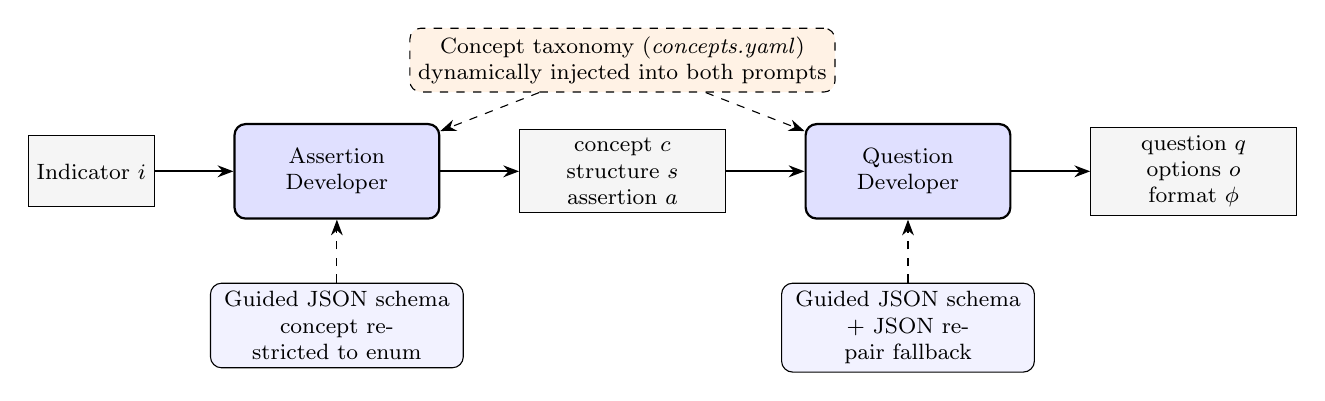
\begin{tikzpicture}[
  node distance=6mm and 10mm,
  font=\footnotesize,
  box/.style={draw, rounded corners, align=center, minimum height=9mm, inner sep=3pt, fill=blue!5},
  agent/.style={draw, thick, rounded corners, align=center, minimum height=12mm, minimum width=26mm, fill=blue!12},
  data/.style={draw, align=center, minimum height=9mm, inner sep=3pt, fill=gray!8},
  ref/.style={draw, dashed, rounded corners, align=center, inner sep=3pt, fill=orange!10},
  flow/.style={-{Stealth[length=2mm]}, thick},
  inject/.style={-{Stealth[length=2mm]}, dashed}
]
\node[data] (ind) {Indicator $i$};
\node[agent, right=of ind] (ad) {Assertion\\Developer};
\node[data, right=of ad, text width=24mm] (astate) {concept $c$\\structure $s$\\assertion $a$};
\node[agent, right=of astate] (qd) {Question\\Developer};
\node[data, right=of qd, text width=24mm] (qstate) {question $q$\\options $o$\\format $\phi$};

\draw[flow] (ind) -- (ad);
\draw[flow] (ad) -- (astate);
\draw[flow] (astate) -- (qd);
\draw[flow] (qd) -- (qstate);

\node[ref, above=10mm of $(ad)!0.5!(qd)$] (yaml) {Concept taxonomy (\emph{concepts.yaml})\\dynamically injected into both prompts};
\draw[inject] (yaml) -- (ad);
\draw[inject] (yaml) -- (qd);

\node[box, below=8mm of ad, text width=30mm] (adc) {Guided JSON schema\\concept restricted to enum};
\node[box, below=8mm of qd, text width=30mm] (qdc) {Guided JSON schema\\+ JSON repair fallback};
\draw[inject] (adc) -- (ad);
\draw[inject] (qdc) -- (qd);
\end{tikzpicture}
\caption{The two-agent pipeline. An indicator is mapped by the Assertion Developer to a concept, structure code, and assertion; the Question Developer then turns an assertion into a question, options, and format. The concept taxonomy is injected into both system prompts at run time, and both stages use schema-guided JSON decoding, with the concept field constrained to the enumerated taxonomy.}
\label{fig:pipeline}
\end{figure*}

\subsection{Dynamic Framework Injection}
Rather than hard-coding the taxonomy into the prompts, we store it in a single machine-readable file (\emph{concepts.yaml}) that lists every concept, its type, and its licensed structure codes, together with the notation key. At run time a prompt loader renders this file into a text block and substitutes it into a placeholder in each agent's system prompt. Consequently the prompts always reflect the current taxonomy, and any change to the framework, such as correcting a licensed code, propagates to both agents without manual prompt edits. This coupling proved important during prompt engineering (Section~\ref{sec:iterations}), where aligning the reference file with the gold labels immediately changed model behavior.

\subsection{Assertion Developer}
The Assertion Developer receives the injected taxonomy and a short instruction to produce an assertion for a given indicator. Its system prompt is organized into four parts: a role description, a set of strict rules (identify exactly one concept, choose only a licensed structure code, output a single declarative sentence, never invent labels), a table of commonly confused concepts with disambiguation rules, and a set of worked examples. The disambiguation table encodes expert heuristics that separate frequently conflated categories, for instance Preference versus Expectations of future events, Action tendencies versus Behaviour, or Place versus Demographics, and it grew over successive prompt iterations as new confusions were observed. The agent returns a JSON object with the fields \emph{concept}, \emph{structure\_code}, and \emph{assertion}. The raw concept string is then mapped to its canonical taxonomy name before scoring, which absorbs superficial spelling differences.

\subsection{Question Developer}
The Question Developer receives an assertion and converts it into a respondent-facing item. Its prompt instructs the model to prefer clear, neutral, direct-interrogative phrasing, to choose a response format appropriate to the concept type (rating scales for subjective concepts; frequency scales, multiple choice, or open-ended formats for objective concepts), and to preserve the meaning of the assertion. It returns a JSON object with the fields \emph{question}, \emph{answer\_options}, and \emph{question\_format}. To keep parsing robust, answer options are required to be a single delimited string rather than a nested list, which avoids a class of malformed-JSON failures observed early in development.

\subsection{Structured Decoding and Robustness}
Both agents use schema-guided JSON decoding: the server is given a JSON schema for the current stage and constrains generation to conform to it. For the Assertion Developer we additionally restrict the \emph{concept} field to an enumeration of the 22 taxonomy names, which makes it impossible for the model to emit an out-of-taxonomy label and removes an entire error mode. A separate schema is used for the Question Developer and, later, for the judge. Two robustness measures handle the remaining failure cases. First, because the base model is a reasoning-capable model that may otherwise emit deliberation text, we disable its thinking mode and append an explicit instruction to return only JSON, which is necessary for reliable structured output. Second, a permissive parser strips any stray text around the JSON object, and a targeted repair routine reconstructs the question fields when the model breaks JSON quoting in the answer-options field.

\subsection{Model and Serving}
Both agents are served by a single instance of an open-weight, instruction-tuned model with roughly nine billion parameters, hosted locally through a high-throughput inference server exposing an OpenAI-compatible API \cite{kwon2023efficient, qwen2024technical}. Generation is deterministic (temperature $0$) with a token budget of $1024$ per call, so that repeated runs of the same prompt are reproducible. The external judge used in Section~\ref{sec:setup} is a larger model from the same family, served separately. Serving open weights locally keeps all data on-premise and fixes the model version across runs; the deployment ran on a single high-memory GPU, with the practical configuration details and workarounds recorded in Appendix~F.


\section{Experimental Setup}
\label{sec:setup}

\subsection{Gold Set}
We evaluate against a hand-built gold set of $115$ items constructed by expert annotation following the framework. Each row specifies an indicator together with its reference concept, structure code, assertion, question, and answer options, and is additionally tagged with an application domain and a subjective/objective marker. Every one of the $22$ basic concepts is represented, so the set exercises the full taxonomy rather than only its common categories. Of the $115$ items, $73$ realize subjective concepts and $42$ realize objective concepts. The items are drawn from roughly $40$ application domains, the most frequent being customer experience, health, employee experience, psychology and education, and social services; the long tail contains many domains represented by a single item, which tests generalization across topics rather than memorization of a narrow area. Table~\ref{tab:gold} reports the per-concept counts.

The distribution is deliberately broad but uneven: frequent concepts such as Evaluation ($n{=}20$) and Demographics ($n{=}15$) are well sampled, whereas a number of concepts, including Norms, Policies, Values, and Causal relationship, appear only three times each. These rare categories yield high-variance per-concept estimates, a caveat we return to in Section~\ref{sec:limitations}, but they are essential for surfacing systematic failure modes on the harder parts of the taxonomy.

\begin{table}[t]
\caption{Gold-Set Composition by Basic Concept ($N=115$)}
\label{tab:gold}
\centering
\footnotesize
\begin{tabular}{l r | l r}
\hline
\textbf{Subjective} & \textbf{n} & \textbf{Objective} & \textbf{n} \\
\hline
Evaluation & 20 & Demographics & 15 \\
Preference & 10 & Behaviour & 7 \\
Cognitive judgement & 7 & Events & 5 \\
Action tendencies & 5 & Knowledge & 3 \\
Feelings & 4 & Time & 3 \\
Importance & 3 & Place & 3 \\
Values & 3 & Quantities & 3 \\
Causal relationship & 3 & Procedures & 3 \\
Similarity relationship & 3 & & \\
Norms & 3 & & \\
Policies & 3 & & \\
Rights & 3 & & \\
Expectations of future events & 3 & & \\
Evaluative belief & 3 & & \\
\hline
\textbf{Subtotal} & \textbf{73} & \textbf{Subtotal} & \textbf{42} \\
\hline
\end{tabular}
\end{table}

\subsection{Isolated Evaluation Protocol}
As motivated in Section~\ref{sec:framework}, the two agents are scored independently. The Assertion Developer is run on the gold indicator, and its predicted concept and structure are compared with the reference. The Question Developer is run on the \emph{gold} assertion rather than the assertion just produced by the first stage, so that a mistake in concept or structure identification cannot contaminate the measurement of question quality. This isolated protocol mirrors the evaluation logic of the framework itself and yields per-stage metrics that are directly attributable to each agent.

\subsection{Normalization}
Objective scoring is exact match after a light normalization that removes differences irrelevant to the framework. Strings are lowercased and stripped of surrounding and internal whitespace before comparison. Concept names are additionally mapped across British and American spelling variants, so that \emph{behavior} and \emph{behaviour}, or \emph{judgment} and \emph{judgement}, are treated as identical.\footnote{The reference file uses British spellings (\emph{Behaviour}, \emph{Cognitive judgement}) while the gold set uses American spellings; the normalization layer reconciles them without editing the source data.} Structure codes are compared after extracting the bare code token with a regular expression, which tolerates incidental annotation such as trailing qualifiers. Crucially, normalization is applied only in the scoring layer; the gold data itself is never modified.

\subsection{Metrics}
We report two families of metrics. The \emph{objective} metrics measure adherence to the framework:
\begin{itemize}
\item \emph{Concept accuracy}: fraction of items whose predicted concept matches the reference after normalization.
\item \emph{Structure accuracy}: fraction whose predicted structure code matches the reference.
\item \emph{Both correct}: fraction for which concept and structure are simultaneously correct, the strictest assertion-stage criterion.
\item \emph{Question coverage}: fraction of items for which a non-empty question is produced, and the fraction for which a question format is assigned.
\item \emph{Question exact match}: fraction whose generated question matches the reference question string after normalization, reported as a strict lower bound on question quality.
\end{itemize}
The \emph{semantic} metrics use an LLM as a judge to rate two alignments on a $1$--$5$ scale: \emph{indicator-to-assertion} (IA), whether the assertion faithfully represents the indicator, and \emph{assertion-to-question} (AQ), whether the question faithfully represents the assertion. The judge is prompted with an explicit rubric (5 = perfect alignment; 4 = minor wording differences; 3 = partial; 2 = poor; 1 = none) and returns a score with a brief rationale, decoded under the judge JSON schema. Judge metrics complement exact match because a generated question may differ in wording from the reference yet still be a faithful, high-quality item.

\subsection{Judge Models}
We use two judge configurations. The \emph{self-judge} is the same 9B model that generates the outputs, which is convenient but risks the self-preference bias discussed in Section~\ref{sec:related}. The \emph{external judge} is a larger, independently served model of roughly $72$ billion parameters from the same family, run on two GPUs. The external judge re-scores the previously generated predictions without any change to prompts or generations, so any difference in scores is attributable to the evaluator rather than to the items being evaluated. Reporting both lets us quantify the self-grading gap directly.

\subsection{Reproducibility}
All runs are driven by a single configuration file that fixes the model paths, decoding parameters (temperature $0$, $1024$ tokens), the judge settings, and the evaluation scope. Because decoding is deterministic, re-running a configuration reproduces its outputs. Each reported run is tied to a specific code state, and the objective summaries and confusion matrices are exported as machine-readable artifacts alongside a per-item prediction table for manual inspection.

\section{Prompt-Engineering Iterations}
\label{sec:iterations}

Rather than tuning the model, we improved the pipeline through a sequence of six controlled iterations, each of which introduced one coherent change while holding the rest of the system fixed. This design lets us attribute changes in accuracy to specific interventions. The interventions fall into three groups: fairer scoring, output constraints, and prompt content (concept and structure disambiguation), plus two judge-only runs that add semantic scoring without altering generations. Table~\ref{tab:changelog} records which technique entered at which run; once introduced, a technique is carried forward.

\begin{table}[t]
\caption{Interventions Introduced at Each Run (Carried Forward Thereafter)}
\label{tab:changelog}
\centering
\scriptsize
\begin{tabular}{l c c c c c c}
\hline
\textbf{Intervention} & \textbf{R1} & \textbf{R2} & \textbf{R3} & \textbf{R4} & \textbf{R5} & \textbf{R6} \\
\hline
Isolated eval; JSON, thinking disabled & \checkmark & & & & & \\
US/UK spelling-normalized scoring & & \checkmark & & & & \\
Concept enum constraint (guided JSON) & & \checkmark & & & & \\
Concept disambiguation table + examples & & \checkmark & & & & \\
Structure disambiguation table + examples & & & \checkmark & & & \\
Question JSON repair fallback & & & \checkmark & & & \\
Confusion matrices + per-category metrics & & & \checkmark & & & \\
Self-judge scoring (9B) & & & & \checkmark & & \\
External judge scoring (72B) & & & & & \checkmark & \\
Structure prompt pass 2 & & & & & & \checkmark \\
Reference file aligned with gold codes & & & & & & \checkmark \\
\hline
\end{tabular}
\end{table}

\emph{Run 1 (initial baseline).} The first full run established the harness: isolated evaluation over all $115$ items, schema-guided JSON decoding with the model's thinking mode disabled, and exact-match scoring with only light string normalization. The assertion prompt contained a role, strict rules, and three worked examples. This run exposed three recurring problems that motivated the next iterations: concept mismatches caused purely by spelling, frequent confusion between related subjective concepts, and occasional malformed question JSON.

\emph{Run 2 (fairer scoring and concept constraints).} Three changes targeted concept identification. Scoring was made spelling-invariant across British and American variants; the predicted concept field was constrained to the enumerated taxonomy so the model could no longer invent labels; and the assertion prompt gained a table of commonly confused concepts with disambiguation rules and three additional worked examples covering those cases. Together these changes chiefly improved concept accuracy.

\emph{Run 3 (structure disambiguation and richer diagnostics).} Attention shifted to structure codes, which lagged concept accuracy. The prompt's brief structure hints were expanded into a full disambiguation table with three further examples, most notably fixing the default structure for Preference. A repair routine recovered question fields when the model broke JSON quoting, eliminating the malformed-output cases. This run also added the diagnostic exports, per-concept and per-structure breakdowns and confusion matrices, that the analysis in Section~\ref{sec:discussion} relies on.

\emph{Run 4 (self-judge).} No prompts or generations changed; the run only enabled LLM-as-judge scoring using the same 9B model, adding the IA and AQ semantic scores. This isolates the effect of adding a semantic metric from any change in the items themselves.

\emph{Run 5 (external judge).} The Run 4 predictions were re-scored by the larger 72B judge, again without regenerating any items. Comparing Run 4 and Run 5 scores on identical outputs measures the self-grading bias directly.

\emph{Run 6 (structure prompt pass 2).} The final iteration addressed the structure codes that remained systematically wrong after Run 3. Two worked examples that had taught incorrect codes were corrected, the disambiguation table was extended with rules for feelings, place and procedures, quantities, time, and the values-versus-importance distinction, and seven new examples were added. Critically, the machine-readable reference file was aligned with the gold structure codes, which, through the dynamic injection of Section~\ref{sec:method}, immediately propagated the corrected codes into the prompt. This run produced the largest single-iteration gain in structure accuracy and is our best configuration.

\section{Results}
\label{sec:results}

We report objective and semantic results for the six runs of Section~\ref{sec:iterations}. Unless noted, ``best'' refers to Run~6, our strongest configuration.

\subsection{Overall Progression}
Table~\ref{tab:main} and Fig.~\ref{fig:progression} summarize the assertion-stage metrics across runs. Prompt engineering alone, with no fine-tuning, raises concept accuracy from $57.4\%$ to $76.5\%$ and structure accuracy from $51.3\%$ to $75.7\%$; the strict both-correct criterion rises from $42.6\%$ to $73.9\%$. The two largest jumps come from the two content interventions: the concept work in Run~2 (concept $+12.2$ points) and the structure pass in Run~6 (structure $+13.1$ points over Run~4). Run~4 reproduces the Run~3 generations exactly and adds only judge scores, so its objective metrics are identical to Run~3.

\begin{table}[t]
\caption{Objective and Semantic Metrics Across Runs (Percent, or 1--5 for Judge Scores)}
\label{tab:main}
\centering
\footnotesize
\begin{tabular}{l c c c c c}
\hline
\textbf{Metric} & \textbf{R1} & \textbf{R2} & \textbf{R3} & \textbf{R4} & \textbf{R6} \\
\hline
Concept accuracy & 57.4 & 69.6 & 75.7 & 75.7$^{*}$ & \textbf{76.5} \\
Structure accuracy & 51.3 & 55.7 & 62.6 & 62.6$^{*}$ & \textbf{75.7} \\
Both correct & 42.6 & 53.0 & 60.9 & 60.9$^{*}$ & \textbf{73.9} \\
Question coverage & 99.1 & 99.1 & 100 & 100 & 100 \\
Question exact match & 20.0 & 20.0 & 18.3 & 18.3 & 17.4 \\
Mean IA (self, 9B) & -- & -- & -- & 4.51 & -- \\
Mean AQ (self, 9B) & -- & -- & -- & 4.99 & -- \\
\hline
\multicolumn{6}{l}{\scriptsize $^{*}$Run 4 re-scores the Run 3 generations; objective metrics are unchanged.}
\end{tabular}
\end{table}

\begin{figure}[t]
\centering
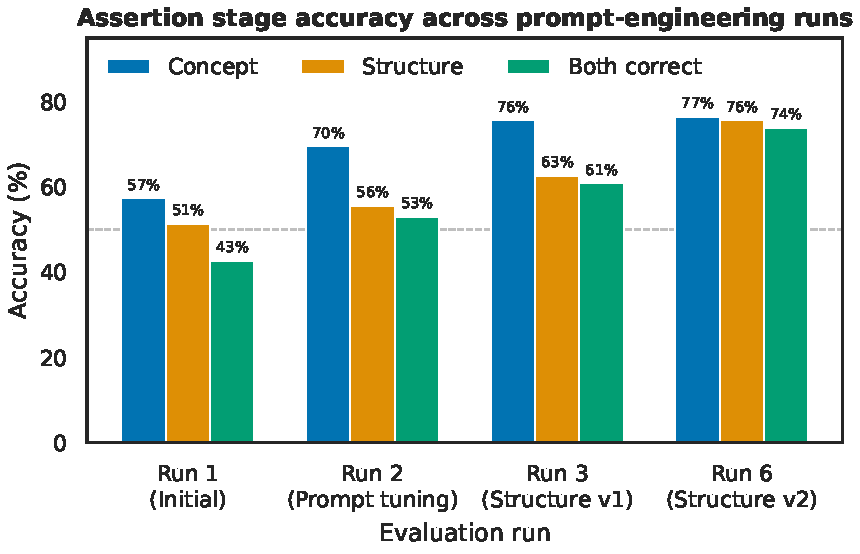
\includegraphics[width=\columnwidth]{fig01_run_progression.pdf}
\caption{Assertion-stage accuracy across the four prompt-engineering runs (Runs 1, 2, 3, and 6; the judge-only runs are omitted). Prompt engineering alone moves concept and structure accuracy from roughly $50\%$ to roughly $76\%$.}
\label{fig:progression}
\end{figure}

\subsection{Per-Concept and Per-Structure Behavior}
Aggregate accuracy hides strong variation across the taxonomy. Fig.~\ref{fig:perconcept} shows per-concept concept and structure accuracy at the best configuration. Seven concepts, including Expectations of future events, Importance, Knowledge, Place, Quantities, Rights, and Time, reach $100\%$ on both concept and structure, while the frequent categories Evaluation, Demographics, and Preference sit at $80\%$. At the other extreme, Norms scores $0\%$ and Policies scores $0\%$ on concept identification, and Causal relationship reaches only $33\%$; these are precisely the rare, semantically subtle categories.

A recurring pattern is a gap between getting the concept right and getting its structure right. Fig.~\ref{fig:gap} plots this directly. Run~6 largely closed the gap for several codes that had been systematically wrong in Run~4: the future-deed code rose from $0\%$ to $88\%$, the place code from $0\%$ to $83\%$, the feeling code from $0\%$ to $75\%$, and the time, quantity, and societal-value codes each reached $100\%$. What remains is concentrated in a few categories where a correct concept is still paired with the wrong structure, discussed in Section~\ref{sec:discussion}.

\begin{figure*}[t]
\centering
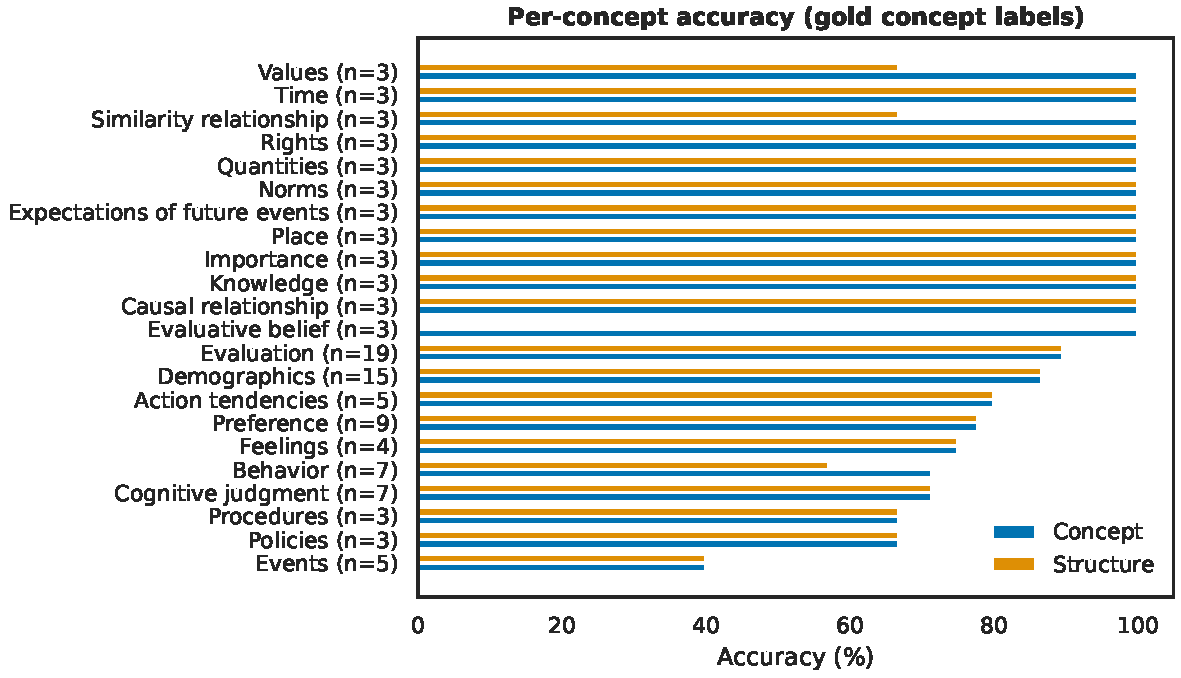
\includegraphics[width=0.86\textwidth]{fig03_per_concept_accuracy.pdf}
\caption{Per-concept concept and structure accuracy at the best configuration (Run 6). Rare, semantically subtle concepts (Norms, Policies, Causal relationship) dominate the errors, while most objective and well-sampled subjective concepts are at or near ceiling.}
\label{fig:perconcept}
\end{figure*}

\begin{figure}[t]
\centering
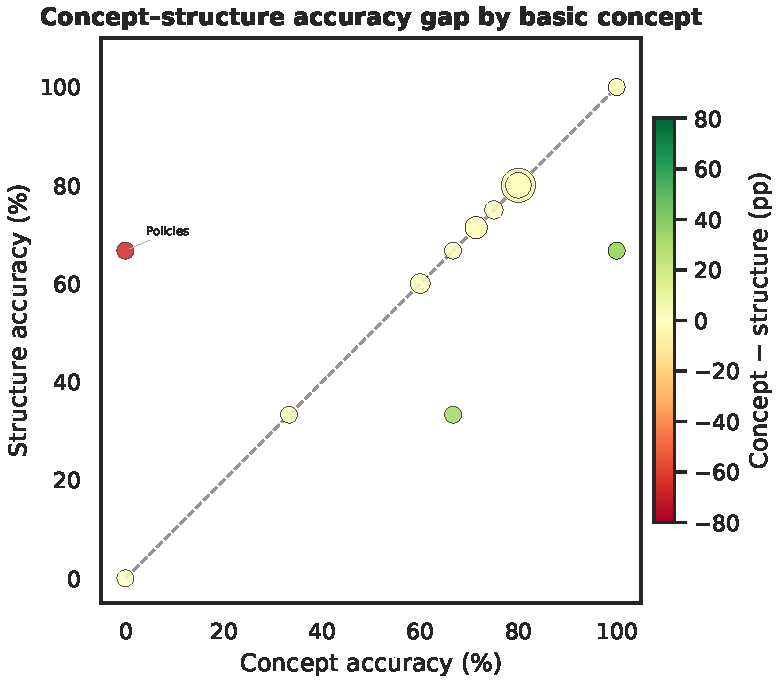
\includegraphics[width=\columnwidth]{fig06_concept_structure_gap.pdf}
\caption{Concept accuracy versus structure accuracy per concept. Points below the diagonal identify concepts the model labels correctly but whose semantic structure it still misassigns.}
\label{fig:gap}
\end{figure}

\subsection{Question Stage}
The Question Developer solves coverage: from Run~3 onward it produces a non-empty question and an assigned format for every item ($100\%$). Exact string match against the reference question, however, is low and slightly decreasing across runs ($20.0\%$ down to $17.4\%$). This is expected: many faithful questions are simply worded differently from the reference. Every generated question was tagged with the same format, a direct interrogative with a WH word, reflecting the prompt's stated preference for that form. Fig.~\ref{fig:exactjudge} contrasts exact match with judge scores and shows that the two are essentially uncorrelated, so exact match understates question quality; the semantic results below make this precise.

\begin{figure}[t]
\centering
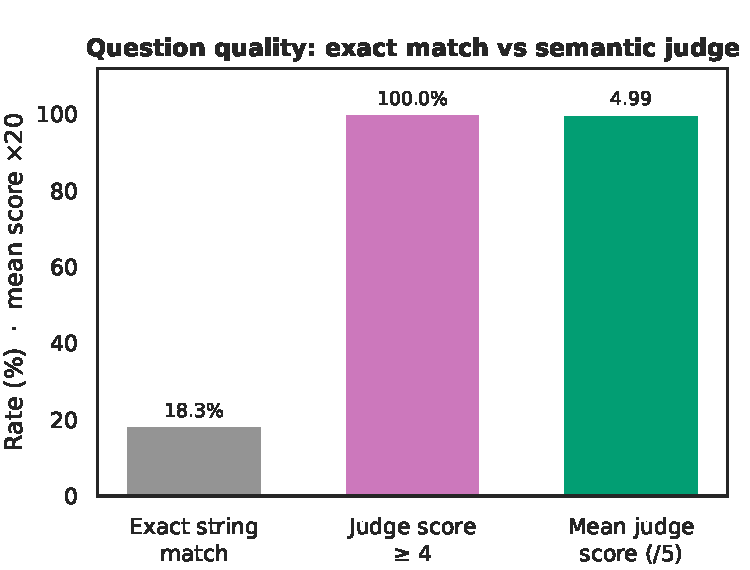
\includegraphics[width=\columnwidth]{fig09_exact_match_vs_judge.pdf}
\caption{Question quality by exact match versus LLM-as-judge. The large majority of questions that do not match the reference wording are nonetheless rated highly aligned, so exact match severely understates quality.}
\label{fig:exactjudge}
\end{figure}

\subsection{Semantic (Judge) Results}
Semantic scoring confirms that both stages are strong. Under the self-judge (Run~4), mean indicator-to-assertion alignment is $4.51/5$ and mean assertion-to-question alignment is $4.99/5$. Re-scoring the identical predictions with the external 72B judge (Run~5) lowers both means, to $4.09$ for IA and $4.56$ for AQ, a drop of roughly $0.43$ points on each metric (Fig.~\ref{fig:selfext}). Despite this correction, the question stage remains strong under the stricter judge: all $115$ items score at least $4$ on assertion-to-question alignment, and $94$ of the $94$ questions that do not exactly match the reference still score at least $4$. The external judge also spreads its scores more realistically than the self-judge, whose IA distribution was sharply bimodal; the external IA distribution is centered on $4$ with a longer lower tail (Fig.~\ref{fig:extdist}). The interpretation of the gap, and of which items the external judge penalizes, is taken up in Section~\ref{sec:discussion}.

\begin{figure}[t]
\centering
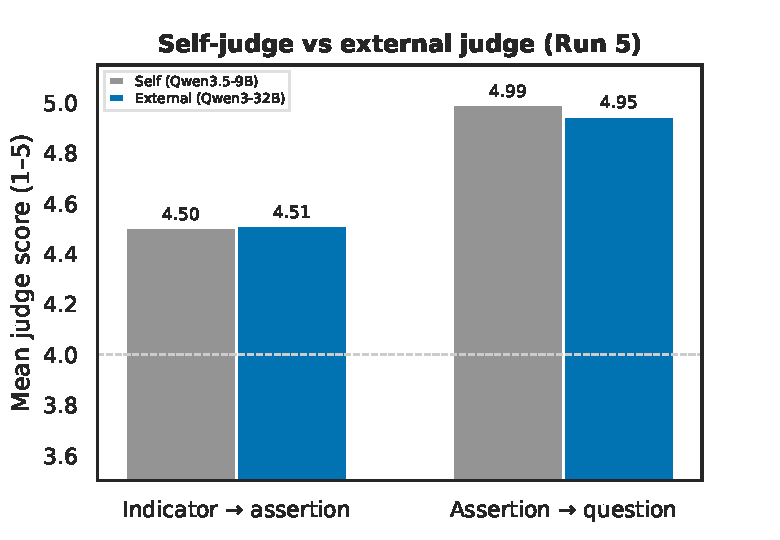
\includegraphics[width=\columnwidth]{fig12_self_vs_external_judge.pdf}
\caption{Mean alignment scores from the self-judge (9B) and the external judge (72B) on identical Run 4 predictions. Both alignments drop by about $0.43$ points under the independent judge, evidence of a self-grading bias.}
\label{fig:selfext}
\end{figure}

\begin{figure}[t]
\centering
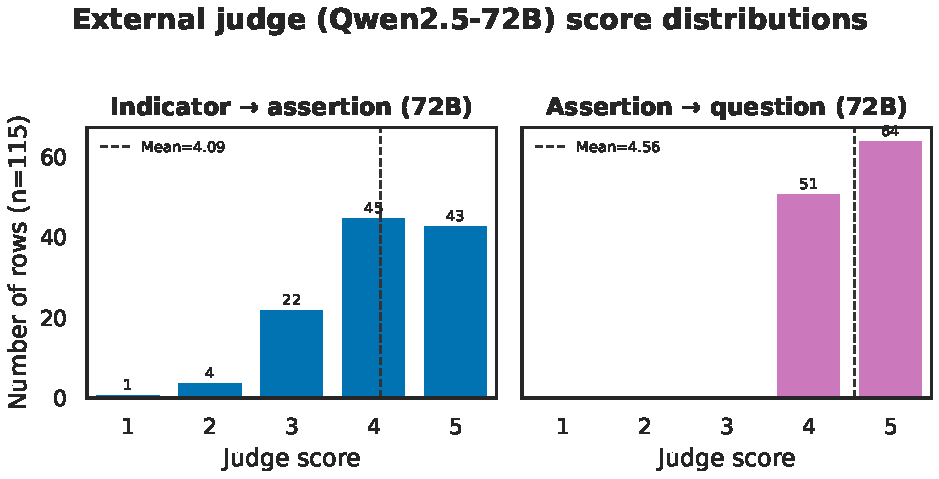
\includegraphics[width=\columnwidth]{fig13_ext_judge_distributions.pdf}
\caption{External-judge (72B) score distributions for indicator-to-assertion and assertion-to-question alignment. Assertion-to-question scores concentrate at 4--5; indicator-to-assertion scores are more spread, with a small low-scoring tail.}
\label{fig:extdist}
\end{figure}


\section{Error Analysis and Discussion}
\label{sec:discussion}

We now examine where the pipeline still fails and what the results imply for automated survey item construction. The confusion structure is analyzed from the per-item predictions of the best configuration; the full confusion matrices are given in Appendix~D, and the most frequent confusions are shown in Fig.~\ref{fig:concconf} and Fig.~\ref{fig:structconf}.

\subsection{Concept Confusions}
The remaining concept errors are not random but cluster on a few semantically adjacent pairs (Fig.~\ref{fig:concconf}). Evaluation is confused with Preference and Feelings when an indicator mixes an appraisal with a desired change; Events are confused with Demographics when a past occurrence is phrased as a static status (for example, a medical condition read as a demographic attribute); and Norms are confused with Values when a deontic ``should'' is read as a statement of what matters in general. These are exactly the distinctions that expert annotators find hardest, and they concentrate on rare concepts where the prompt provides few or no worked examples.

\begin{figure}[t]
\centering
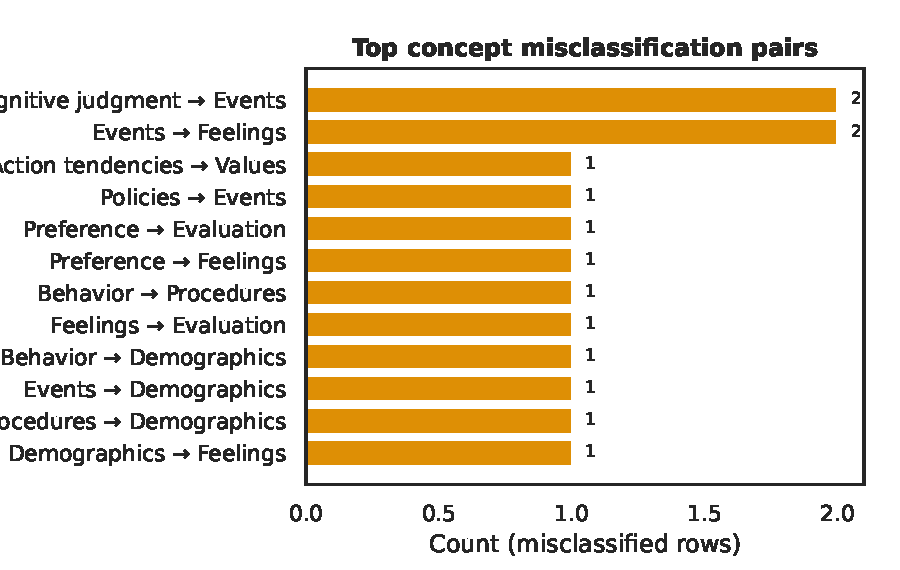
\includegraphics[width=\columnwidth]{fig07_top_concept_confusions.pdf}
\caption{Most frequent concept misclassification pairs at the best configuration. Errors concentrate on semantically adjacent categories rather than being spread uniformly.}
\label{fig:concconf}
\end{figure}

\subsection{Structure Confusions and the Concept--Structure Coupling}
Structure errors have two distinct sources (Fig.~\ref{fig:structconf}). The first is coupling: when the concept is wrong, the structure is almost always wrong too, because the licensed codes differ between concepts. The second, more interesting, source is cases where the concept is correct but the structure is not. Before Run~6 this was systematic: Expectations of future events reached full concept accuracy while its structure code was consistently wrong, and similar behavior appeared for action tendencies and feelings. Aligning the reference file with the gold codes and correcting two misleading examples removed most of these errors at once. What remains are a handful of within-concept structure slips, for example the evaluative-belief predicate code, the values-versus-importance code, and the similarity code, each affecting only one or two items.

\begin{figure}[t]
\centering
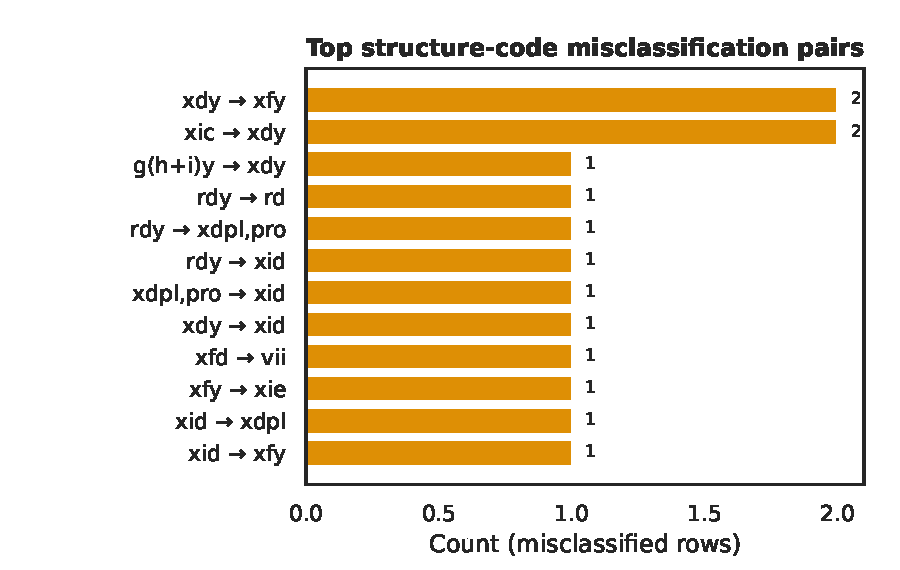
\includegraphics[width=\columnwidth]{fig07_top_structure_confusions.pdf}
\caption{Most frequent structure-code misclassification pairs. Many are induced by an upstream concept error; the rest are within-concept slips on a small number of codes.}
\label{fig:structconf}
\end{figure}

\subsection{A Prompt-Engineering Trade-off: The Norms Regression}
Prompt engineering is not monotonic. The Run~6 pass that strengthened the values-versus-importance rules had a side effect: the model began mapping deontic ``should'' and ``ought'' indicators to Values rather than Norms, so the Norms code, previously correct, regressed to $0\%$. This is a concrete illustration that reinforcing one distinction can weaken an adjacent one when categories share surface cues, and it argues for adding a targeted Norms example rather than further broadening the values rule. We treat this as the clearest next prompt fix.

\subsection{Self- versus External-Judge Bias}
The self-judge and external judge agree on the qualitative conclusions but not on the numbers. Both alignment scores fall by about $0.43$ points under the independent 72B judge, confirming a self-grading bias in which the 9B model rates its own outputs generously. The bias is not uniform: the largest self-minus-external gaps cluster on Demographics indicators, where the external judge penalizes first-person paraphrases (for example, rendering an employment-status or household-composition indicator as ``My employment status is\ldots'') as a scope mismatch for what should be a neutral factual item, whereas the self-judge rated them perfect. The external judge also discriminates more sharply by correctness: its mean indicator-to-assertion score is clearly lower when the concept label is wrong than when it is right, a separation the self-judge largely failed to make. This is direct evidence for reporting an independent judge rather than self-evaluation.

\subsection{Exact Match Understates Question Quality}
The question stage exposes a measurement pitfall. Exact string match against the reference is low (about $17\%$) and is essentially uncorrelated with judged alignment. Under the external judge, every non-matching question that we examined still scored at least $4$ on assertion-to-question alignment. In other words, exact match here measures wording overlap, not quality, and would badly misrank the system. For generative item construction we therefore recommend judge-based alignment as the primary question metric, with exact match reported only as a strict, conservative lower bound.

\subsection{Prompt Engineering versus Fine-Tuning}
Taken together, the results show that framework-grounded prompt engineering reaches roughly $76\%$ on both concept and structure identification, and near-ceiling semantic quality on the question stage, without any parameter updates. The residual errors are concentrated on a small number of rare, semantically subtle concepts (Norms, Policies, Causal relationship), each represented by only three gold items. Because these categories are both rare and hard, the highest-value next step is targeted: additional worked examples for the deontic and causal concepts, before considering parameter-efficient fine-tuning. Fine-tuning is thus better seen as an optional refinement for the long tail than as a prerequisite for a strong baseline.

\section{Limitations}
\label{sec:limitations}

Several limitations bound the scope of our conclusions. First, the gold set is small: $115$ items, with a number of concepts represented by only three examples each. Per-concept accuracies for these rare categories are therefore high-variance point estimates, and small absolute changes should not be over-interpreted. Second, all generation uses a single open-weight model family; while the external judge is from the same family at a larger scale, we do not test whether the findings transfer to other model families, and using a same-family judge may understate cross-family disagreement. Third, our semantic evaluation relies on an LLM judge. We quantify and partly correct for self-grading bias by using an independent, larger judge, but we do not yet validate either judge against expert human ratings, so the absolute alignment scores should be read as model-based estimates rather than ground truth. Fourth, the evaluation scores each stage in isolation and on single-facet indicators; it does not measure end-to-end behavior on broad or compound indicators, nor downstream data-quality outcomes such as respondent comprehension or measurement validity. Finally, the gold set and prompts are English-only, and the framework's concept and structure taxonomy, though general in intent, is applied here within that single-language setting.

\section{Conclusion and Future Work}
\label{sec:conclusion}

We presented a framework-grounded, two-agent pipeline that turns raw indicators into survey items by following a formal three-step design method, using constrained decoding to keep every output inside the concept-and-structure taxonomy. Evaluated against a $115$-item expert gold set with a dual protocol that separates framework adherence from semantic fidelity, the pipeline reaches $76.5\%$ concept accuracy and $75.7\%$ structure accuracy through prompt engineering alone, with both labels jointly correct on $73.9\%$ of items and near-ceiling question quality confirmed by an independent judge ($4.56/5$ assertion-to-question alignment, all items at least $4$). Along the way we showed that exact string match badly understates generative question quality, and we quantified a roughly $0.43$-point self-grading bias that motivates reporting an independent judge.

Three directions follow directly from the error analysis. The most immediate is a targeted prompt fix for the concepts, adding worked examples that separate Norms from Values to repair the regression introduced by the final structure pass, and, more broadly, examples for Policies and Causal relationship, the categories that dominate the residual errors. Second, the semantic evaluation should be extended by re-scoring the best configuration with the external judge and by validating the judge against a modest set of expert human ratings, so that the alignment scores can be calibrated. Third, parameter-efficient fine-tuning on the rare concepts is a natural refinement once prompt-based gains plateau, though our results indicate it is optional rather than necessary for a strong baseline. More broadly, the combination of taxonomy-grounded generation and a dual, bias-aware evaluation offers a reusable template for applying large language models to other structured measurement tasks in computational social science.

\appendices

\section{Notation Key}
\label{app:notation}
Table~\ref{tab:notation} lists the symbols used to build the structure codes of Section~\ref{sec:framework}. A code concatenates a subject symbol, a linking element, and, where present, an object or complement symbol; the three base templates are given in Table~\ref{tab:structures}.

\begin{table}[ht]
\caption{Structure-Code Notation}
\label{tab:notation}
\centering
\footnotesize
\begin{tabular}{c l}
\hline
\textbf{Symbol} & \textbf{Meaning} \\
\hline
$x$ & grammatical subject (respondent or topic) \\
$r$ & respondent as actor \\
$o$ & generic / anyone as subject \\
$g$ & government as subject \\
$I$ & link verb (is / are / was) \\
$P$ & predicator (general) \\
$C$ & causal relationship (subject causes object) \\
$D$ & deed / action \\
$F$ & feeling \\
$FD$ & future deed \\
$H({+}I)$ & has to / should + infinitive \\
$HR$ & has the right to \\
$PR$ & preference \\
$S$ & similarity or difference \\
$e$ & evaluative adjective \\
$i$ & importance adjective \\
$f$ & feeling noun / adjective \\
$c$ & cognitive judgement \\
$ca$ & causal marker \\
$s$ & similarity marker \\
$pr$ & preference marker \\
$ri$ & rights marker \\
$d$ & demographic descriptor \\
$sc$ & scale / classifier \\
$ti$ & time expression \\
$pl$ & place expression \\
$qu$ & quantity expression \\
$pro$ & procedure expression \\
$y$ & object / second entity \\
$z$ & comparison referent \\
\hline
\end{tabular}
\end{table}

\section{Agent Prompts}
\label{app:prompts}
Both prompts begin with the dynamically injected taxonomy block (Section~\ref{sec:method}); only the fixed portions are reproduced here in abbreviated form.

\emph{Assertion Developer.} Role: an expert survey methodologist that converts a raw indicator into a theory-grounded assertion. Strict rules: (1) identify exactly one basic concept, using its exact taxonomy name; (2) choose only a structure code licensed for that concept; (3) output a single declarative sentence following that structure; (4) keep the sentence natural and respondent-appropriate; (5) never invent concepts or codes; (6) apply the disambiguation rules when the indicator is ambiguous; (7) output only a JSON object with keys \emph{concept}, \emph{structure\_code}, \emph{assertion}. The prompt then supplies a ``commonly confused concepts'' table (for example, Evaluation vs.\ Evaluative belief; Expectations of future events vs.\ Action tendencies; Place vs.\ Demographics), a structure-disambiguation table keyed by code, and sixteen worked examples. A representative example: indicator ``repurchase intention'' maps to concept Action tendencies, code $xFD$, assertion ``I intend to purchase from this organization again.''

\emph{Question Developer.} Role: an expert questionnaire designer that turns an assertion into a question and answer options. Rules: convert the declarative assertion into a clear, neutral question; prefer direct-interrogative phrasing; select a response format appropriate to the concept type (rating scales for subjective concepts; frequency, multiple-choice, or open-ended for objective ones); preserve meaning; return answer options as a single delimited string; and output only a JSON object with keys \emph{question}, \emph{answer\_options}, \emph{question\_format}. A representative example: assertion ``I am satisfied with this product'' maps to question ``How satisfied are you with this product?'', a rating scale, tagged as a direct interrogative.

\section{Complete Per-Concept Results}
\label{app:perconcept}
Table~\ref{tab:perconcept} reports concept and structure accuracy for all $22$ concepts at the best configuration (Run~6), with gold-set counts.

\begin{table}[ht]
\caption{Per-Concept Accuracy at the Best Configuration (Run 6)}
\label{tab:perconcept}
\centering
\footnotesize
\begin{tabular}{l r r r}
\hline
\textbf{Concept} & \textbf{n} & \textbf{Concept \%} & \textbf{Structure \%} \\
\hline
\multicolumn{4}{l}{\emph{Subjective}} \\
Evaluation & 20 & 80.0 & 80.0 \\
Preference & 10 & 80.0 & 80.0 \\
Cognitive judgement & 7 & 71.4 & 71.4 \\
Action tendencies & 5 & 80.0 & 80.0 \\
Feelings & 4 & 75.0 & 75.0 \\
Importance & 3 & 100.0 & 100.0 \\
Values & 3 & 100.0 & 66.7 \\
Causal relationship & 3 & 33.3 & 33.3 \\
Similarity relationship & 3 & 100.0 & 66.7 \\
Norms & 3 & 0.0 & 0.0 \\
Policies & 3 & 0.0 & 66.7 \\
Rights & 3 & 100.0 & 100.0 \\
Expectations of future events & 3 & 100.0 & 100.0 \\
Evaluative belief & 3 & 66.7 & 33.3 \\
\hline
\multicolumn{4}{l}{\emph{Objective}} \\
Demographics & 15 & 80.0 & 80.0 \\
Behaviour & 7 & 71.4 & 71.4 \\
Events & 5 & 60.0 & 60.0 \\
Knowledge & 3 & 100.0 & 100.0 \\
Time & 3 & 100.0 & 100.0 \\
Place & 3 & 100.0 & 100.0 \\
Quantities & 3 & 100.0 & 100.0 \\
Procedures & 3 & 66.7 & 66.7 \\
\hline
\end{tabular}
\end{table}

\section{Confusion Matrices}
\label{app:confusion}
Fig.~\ref{fig:concheat} and Fig.~\ref{fig:structheat} give the full concept and structure confusion matrices at the best configuration, from which the most frequent confusions in Section~\ref{sec:discussion} are drawn.

\begin{figure}[ht]
\centering
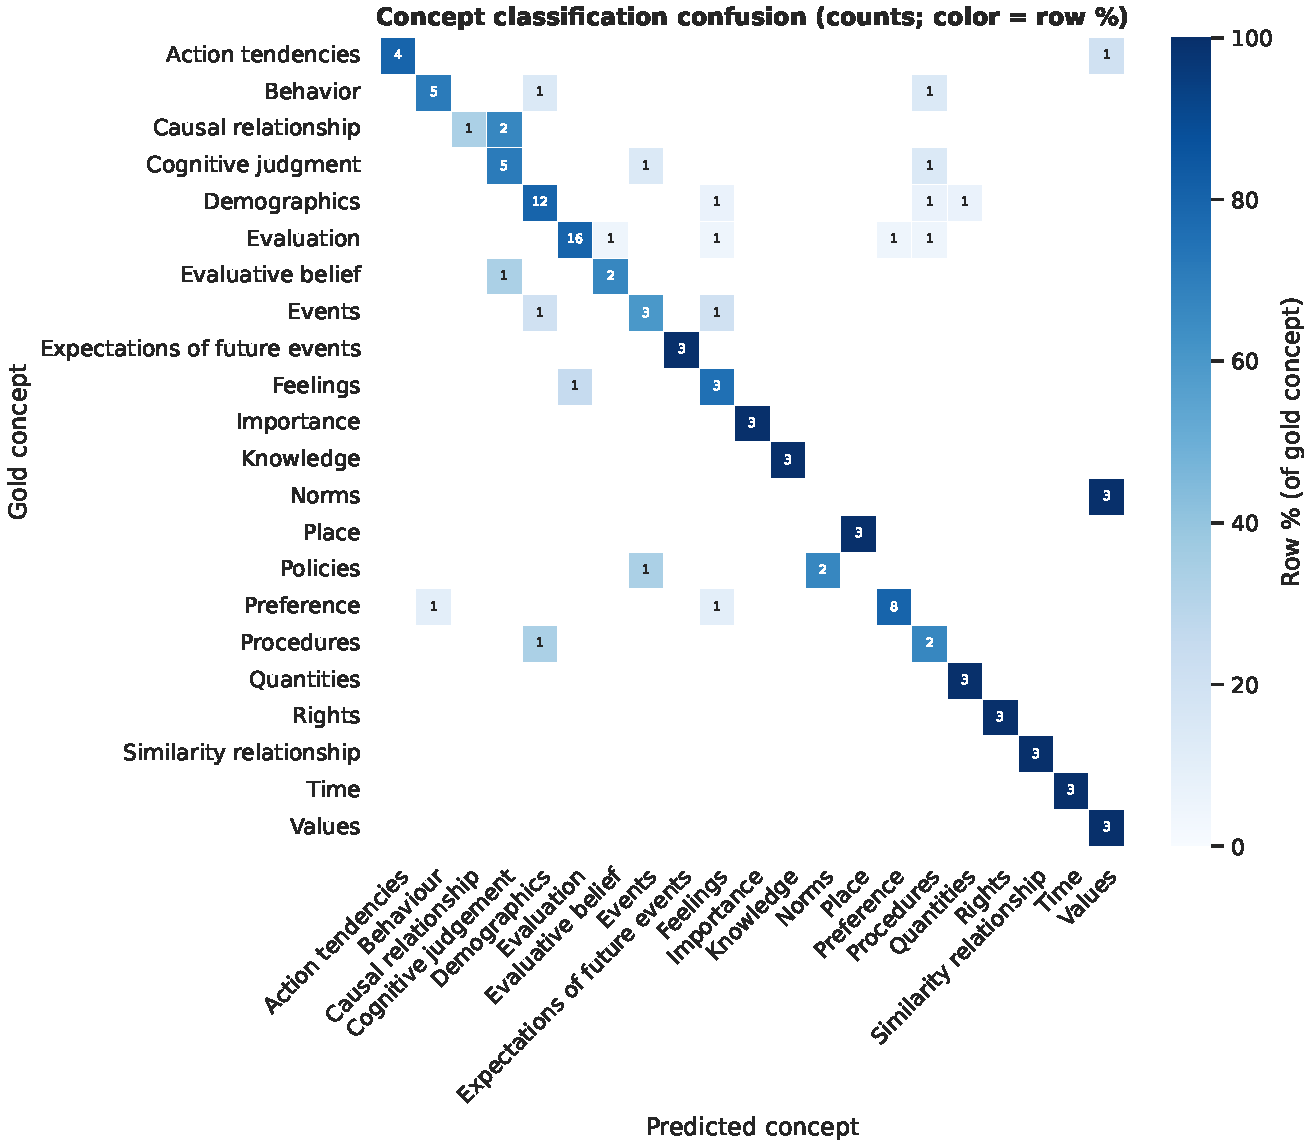
\includegraphics[width=\columnwidth]{fig04_concept_confusion_heatmap.pdf}
\caption{Concept confusion matrix (Run 6). Rows are gold concepts, columns are predictions; color encodes row-normalized rate.}
\label{fig:concheat}
\end{figure}

\begin{figure}[ht]
\centering
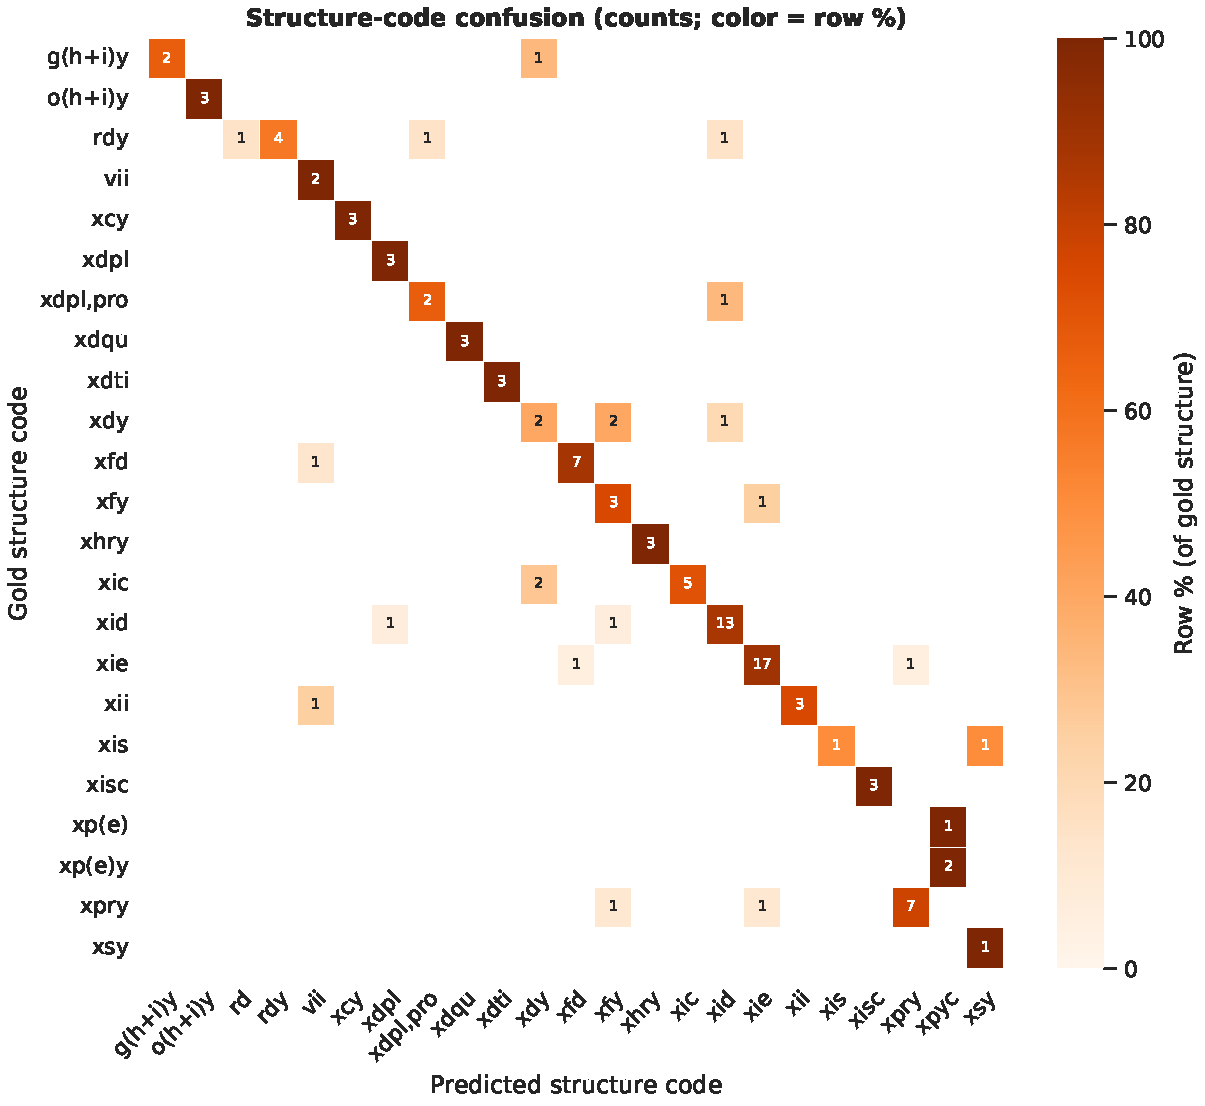
\includegraphics[width=\columnwidth]{fig05_structure_confusion_heatmap.pdf}
\caption{Structure-code confusion matrix (Run 6).}
\label{fig:structheat}
\end{figure}

\section{Judge Rubric and Hardest Items}
\label{app:judge}
The judge is prompted with a fixed rubric on a $1$--$5$ scale: $5$ perfect alignment; $4$ minor wording or format differences only; $3$ partial alignment, related but missing nuance or scope; $2$ poor alignment, significant mismatch; $1$ no alignment. It returns a score and a brief rationale under the judge JSON schema. Table~\ref{tab:worst} lists the items with the lowest external indicator-to-assertion scores, most of which coincide with concept errors and with first-person phrasings of factual indicators; the last row also illustrates the self-judge over-rating an item the external judge scored low.

\begin{table}[ht]
\caption{Hardest Items by External Indicator-to-Assertion Score}
\label{tab:worst}
\centering
\footnotesize
\begin{tabular}{l l c c}
\hline
\textbf{Indicator} & \textbf{Error} & \textbf{Ext} & \textbf{Self} \\
\hline
Medication details & Procedures $\to$ Demographics & 1 & 1 \\
Average stress level & Feelings, wrong structure & 2 & 2 \\
Medical conditions & Events $\to$ Demographics & 2 & 2 \\
Areas for improvement & Evaluation $\to$ Preference & 2 & 2 \\
Length of engagement & Time $\to$ Demographics & 2 & 5 \\
\hline
\end{tabular}
\end{table}

\section{Reproduction Details}
\label{app:repro}
Generation and judging use an OpenAI-compatible inference server hosting the open-weight models locally on GPU. The generator runs on a single high-memory GPU; the 72B external judge runs on two GPUs with tensor parallelism. Decoding is deterministic (temperature $0$, up to $1024$ tokens per call). For reliable structured output from the reasoning-capable base model, thinking mode is disabled and an explicit instruction to emit only JSON is appended to each request; both stages use schema-guided JSON decoding, and the assertion stage additionally constrains the concept field to the enumerated taxonomy. On the target hardware the server required a non-default attention backend and eager execution to run stably; the exact backend flags, library-path ordering, and launch scripts are provided with the code release. Runs are configuration-driven, so fixing the configuration file and model version reproduces the reported outputs, and each run additionally exports a per-item prediction table together with the objective summary and confusion matrices.



\bibliographystyle{ieeetr}
\bibliography{references}

\end{document}
